% #############################################################################
% This is Chapter 3
% !TEX root = ../main.tex
% #############################################################################
% Change the Name of the Chapter i the following line
\fancychapter{Proposed research framework and building specifications}
\cleardoublepage
% The following line allows to ref this chapter
\label{chap:architecture}


In the last chapter we presented some of the most important models in the literature regarding the forecast of energy consumption of buildings. In this chapter we will present in more detail the challenge proposed by \ac{EDP} and the specifications of the building used in this case study, as well as the framework used to address this problem.

\section{Problem statement}

The proposed theme for this work is to create a model capable of making predictions regarding the power profile of the building in question. The data obtained through the proposed model will then be used as input for an optimization system that is outside the scope of this thesis. Since the work to be developed is directly associated with the behavior of the building, it then makes sense to present the building and its characteristics.



\section{The building}\label{subbuild}

As previously mentioned, the work developed during this thesis was based on the development of a system to be applied to a particular building. It makes sense then to describe the building in question and refer to some of its specifications, relevant for the development of this work.

The building provided by \ac{EDP} for this work has a total useful area of $39,801m^2$ distributed in 5 major categories, office area, parking area, technical area, gymnasium area and bar, with the first two areas representing 89\% of the total area of the building. In Figure \ref{consedp} there is a graph that shows the distribution of energy consumption by type of final use in each area of the building.

\begin{figure}[h!]
    \centering
    \begin{center}
    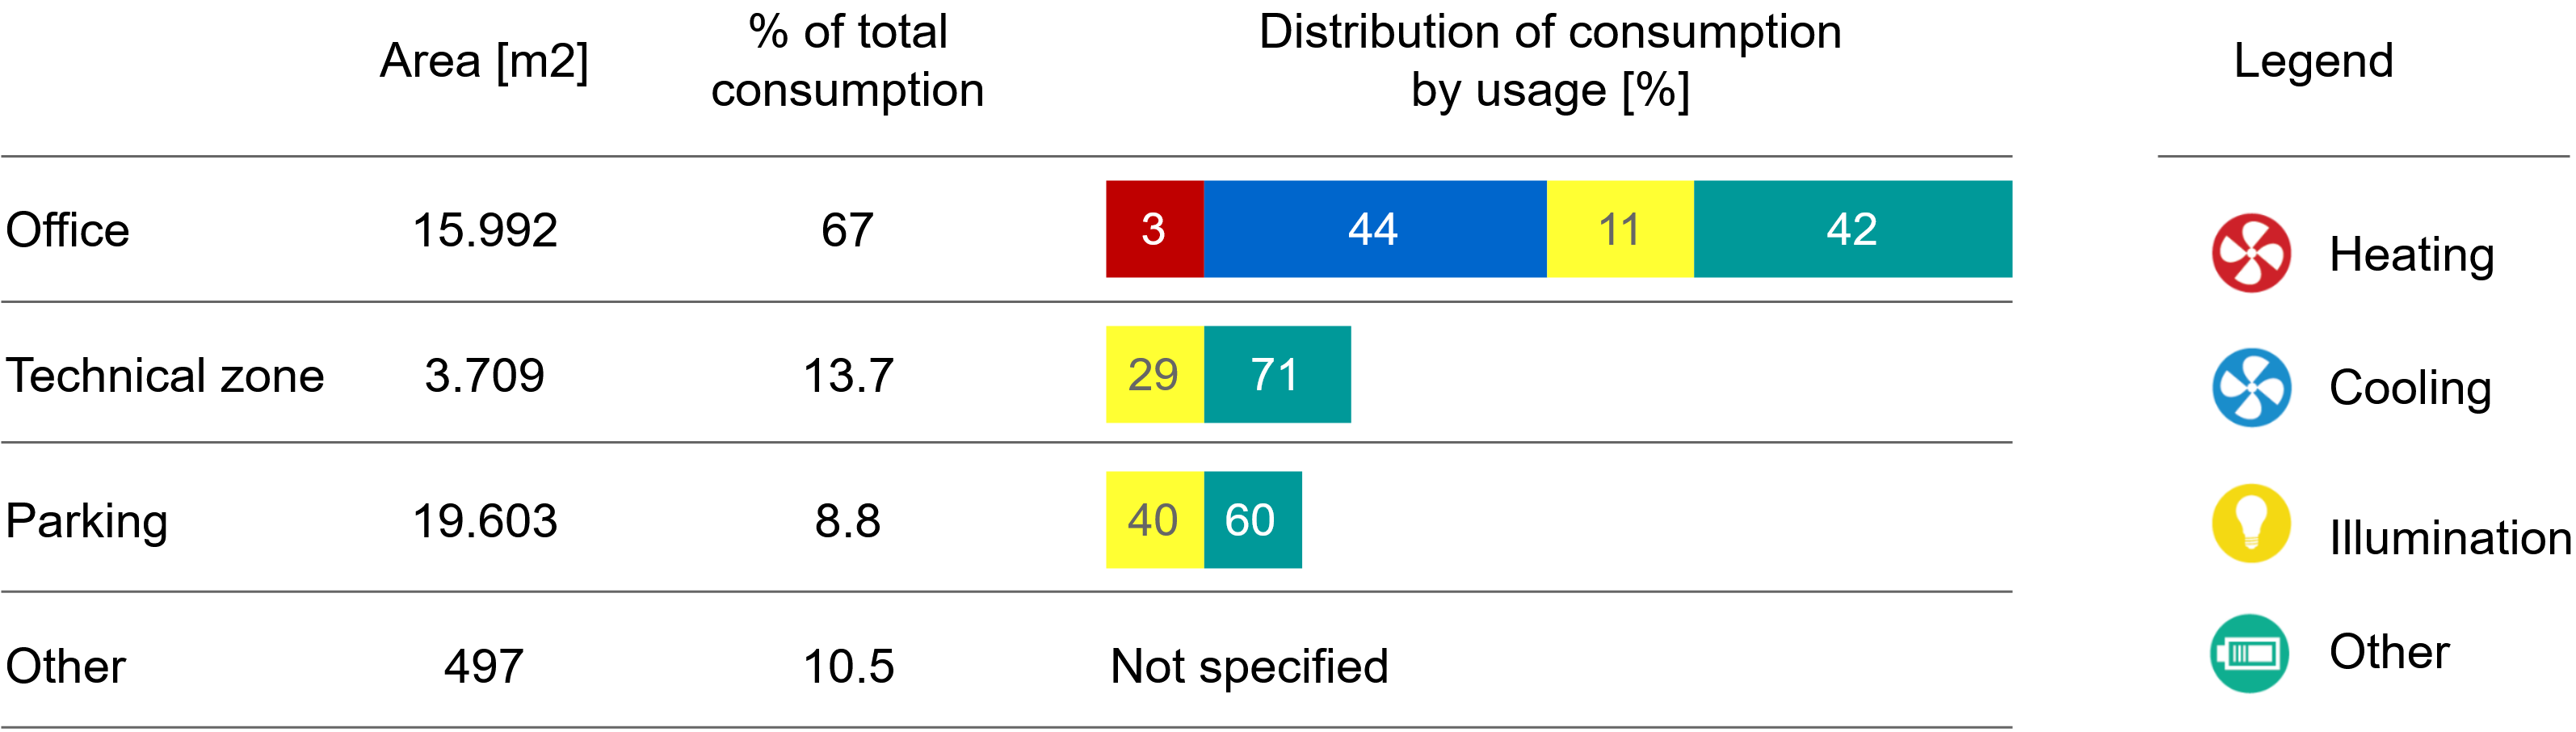
\includegraphics[width=1\textwidth]{Images/ConsumoEDP.png}
    \caption{Energy consumption for the building typology(s) with the highest consumption.}
    \label{consedp}
    \end{center}
\end{figure}
In Figure \ref{consedp} it can be seen that the \ac{HVAC} system represents almost 50\% of the consumption in the office zone. The utilization of the \ac{HVAC} system is directly related to the external weather conditions. In contrast to the commercial buildings explored in section \ref{c}, since 44\% of the consumption is connected to the office cooling process, it can be deduced that in the region where this building is located and in warmer years, the consumption of the office area is higher, contributing to an increase in the total consumption of the building. It can also be seen that only 11\% of consumption is due to the lighting of the office area. On the other hand, 42\% of the consumption in the office area is made up of all other factors such as energy plugs. The technical zones represent about 14\% of the total consumption of the building although they represent a small portion of the total area of the building. Most of the consumption performed in these areas is identified as "other" and concerns servers and technical material of the high energy consumption, hence the enormous representativeness of these zones in the total consumption of the building. Parking lots also represent a significant portion of the total consumption of the building. It should be noted that 60\% of consumption is also identified as "other". This portion mainly concerns the electric car loading that is carried out in the building's garage, managed by the “\ac{EV} Smart Charging Central System", addressed in Chapter \ref{chap:intro}.

\section{Proposed framework}\label{propfram}
During this study, the work had to be divided into several phases in order to respond to the proposed problem. In Figure \ref{framework}, the reader can observe a state map where the step-by-step identification of the different stages of development of this thesis can be found.

\begin{figure}[h!]
    \centering
    \begin{center}
    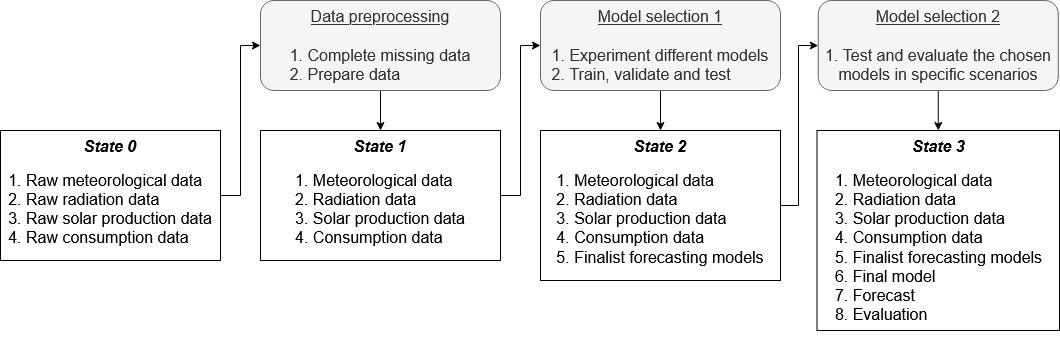
\includegraphics[width=1\textwidth]{Images/framework.png}
    \caption{Proposed research framework.}
    \label{framework}
    \end{center}
\end{figure}

In state 0, one starts only with raw data, where some of the datasets were incomplete, so one of the first challenges was to develop some methods to complete the missing data. In addition, in this section it was also necessary to understand which data was relevant to enter as input in the models, as well as to limit all the data to a specific time window in order to obtain a time interval in which the four datasets were complete. In state 1 the datasets are complete and the data is analyzed and prepared so that it can be introduced as input in the models to be tested. It is in this section that are also decided which variables to use in order to optimize the results of the models. Afterwards different models are built, they are trained, validated and tested, and in state 2 they already have the first forecast results for the models that presented the best performance in the first set of tests. The best or the best model are then chosen, and different tests are carried out to understand what the behavior of the chosen model is in relation to certain situations. In state 3, we have the results obtained by the best models, as well as an evaluation of their performance in general.

\section{Conclusion}

This chapter can be divided into two parts, in the first part, sub-chapter \ref{subbuild}, some relevant data regarding the building used in the case study portrayed in this thesis are identified. In the second part, sub-chapter \ref{propfram} is made a schematization of the work developed in order to facilitate the understanding of the chapters that follow.